\documentclass[11pt,a4paper]{report}

\usepackage[T1]{fontenc}
\usepackage[utf8]{inputenc}
\usepackage[english]{babel}
\usepackage{lmodern}
%\usepackage{circuitikz}
\usepackage{color}
\usepackage{wrapfig}
\usepackage{placeins}
\usepackage{subfigure}
\usepackage{tabu}
\usepackage{fullpage}
\usepackage[squaren]{SIunits}
\usepackage{graphicx}
%\usepackage[pdftex]{graphicx}
\usepackage{epstopdf}
\usepackage{epsfig}
\usepackage{hyperref}
\usepackage{tikz}
\usepackage{tikz-qtree}
\usepackage{eurosym}
%\usepackage{chemist}
\usepackage{amsmath}
\usepackage{amssymb}
\usepackage{mathrsfs}
\usepackage{dsfont}% use $\mathds{1}$
\newcommand{\C}{\mathbb{C}}
\newcommand{\N}{\mathbb{N}}
\newcommand{\Z}{\mathbb{Z}}
\newcommand{\R}{\mathbb{R}}
\newcommand{\red}{\textcolor{red}}
\newcommand{\dis}{\displaystyle}
\newcommand{\dr}{\partial}
\newcommand{\txt}{\text}
\newcommand{\td}{\todo[inline]}
\newcommand{\ttt}{\texttt}
\newcommand{\itt}{\textit}

\usepackage{algorithm}
\usepackage{todonotes}
\usepackage[noend]{algpseudocode}

%\newtheorem{theoreme}			     {Théorème}	[chapter]
%\newtheorem{proposition}[theoreme]	 {Proposition}	
%\newtheorem{corollaire}	  [theoreme]	 {Corollaire}	
%\newtheorem{lemme}	      [theoreme]  {Lemme}		
%\newtheorem{definition}	         {Définition}[chapter]
%\theoremstyle{definition}
%\newtheorem{exemple}			     {Exemple}	[chapter]
%\newtheorem{contreexemple}[exemple]{Contre-exemple}
%\newtheorem{probleme}	             {Probl\`eme}[chapter]

\usepackage{listings}
\usepackage{textcomp}
\definecolor{listinggray}{gray}{0.9}
\definecolor{lbcolor}{rgb}{0.9,0.9,0.9}
\lstset{
	backgroundcolor=\color{lbcolor},
	tabsize=4,
	rulecolor=,
	language=matlab,
        basicstyle=\scriptsize,
        upquote=true,
        aboveskip={1.5\baselineskip},
        columns=fixed,
        showstringspaces=false,
        extendedchars=true,
        breaklines=true,
        prebreak = \raisebox{0ex}[0ex][0ex]{\ensuremath{\hookleftarrow}},
        frame=single,
        showtabs=false,
        showspaces=false,
        showstringspaces=false,
        identifierstyle=\ttfamily,
        keywordstyle=\color[rgb]{0,0,1},
        commentstyle=\color[rgb]{0.133,0.545,0.133},
        stringstyle=\color[rgb]{0.627,0.126,0.941},
}

\DeclareMathOperator{\e}{e}

\title{Titre}
\author{Florentin Goyens}
\date{\today}

\begin{document}
\tabulinesep=1.2mm
\begin{center}
\hrule
\begin{tabular}{c}
\\[0.005cm]
\Large{Applied Numerical Methods - Lab 4}\\[0.3cm]
\textsc{Goyens} Florentin  \& \textsc{Weicker} David\\[0.2cm]
$\text{6}^{\text{th}}$ November 2015\\[0.2cm]
\end{tabular}
\hrule
\end{center}


\section*{Stationary heat conduction in 1-D}

In a one dimensional pipe we are interested in the temperature evolution along the z-axis.  We will study the behaviour of the numerical solution based on finite differences.



\subsection*{a) Reformulation of the problem}

Bla bla bla

\subsection*{b) Discretize to a system of equation}

Bla bla bla

\subsection*{c) Resolution}

Bla bla bla

\subsection*{d) Comparison of methods}

bla bla bla

Ceci est la partie d

\subsection*{e) Improvements}

Ceci est la partie e

\subsection*{f) Visualization}

This section is about the visualization of the results. The Matlab code can be found at the end of the report. Figure \ref{four} shows the temperature in the rod at four time points (namely $\tau \approx 0.5,1,1.5,2$).

\begin{figure}
\begin{center}
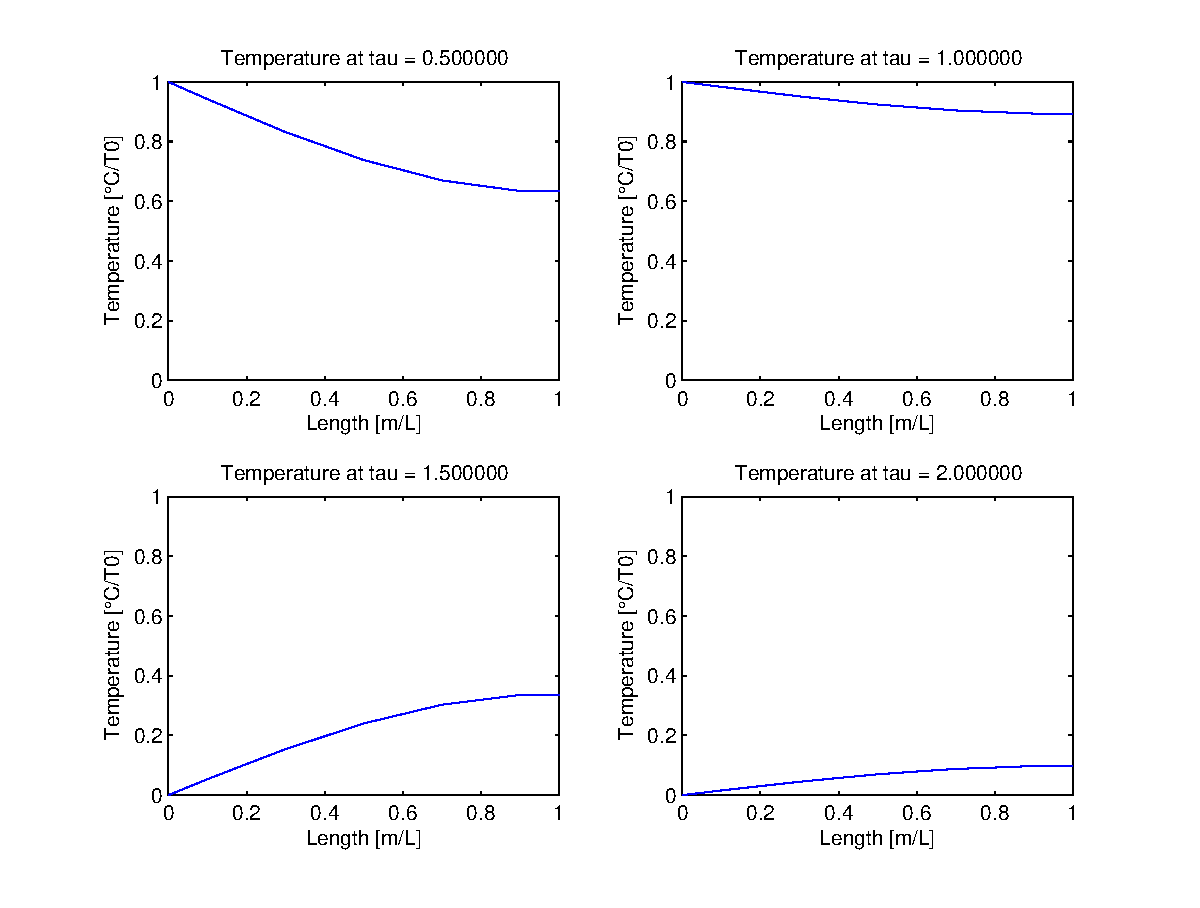
\includegraphics[width=0.9\textwidth]{four.eps}
\caption{Temperature in the rod at different times}
\label{four}
\end{center}
\end{figure}

We can notice that the boundary condition is fulfilled (as it always should be). The temperature rises until $\tau = 1$ and then starts decreasing, as it is expected. 

The next plot is the same as the stable one in section c). It is shown in figure \ref{stable}. This plot clearly depicts the boundary condition. As for the initial condition, the discretization of the $x$-axis has made it less obvious. We have in fact $u(0,0)=1$ and $u(0.1,0) = U_1(0) = 0$. Between the two, it should be zero but Matlab uses a linear interpolation. We can also see here that until $\tau=1$, the temperature is rising while it is decreasing afterwards.

\begin{figure}
\begin{center}
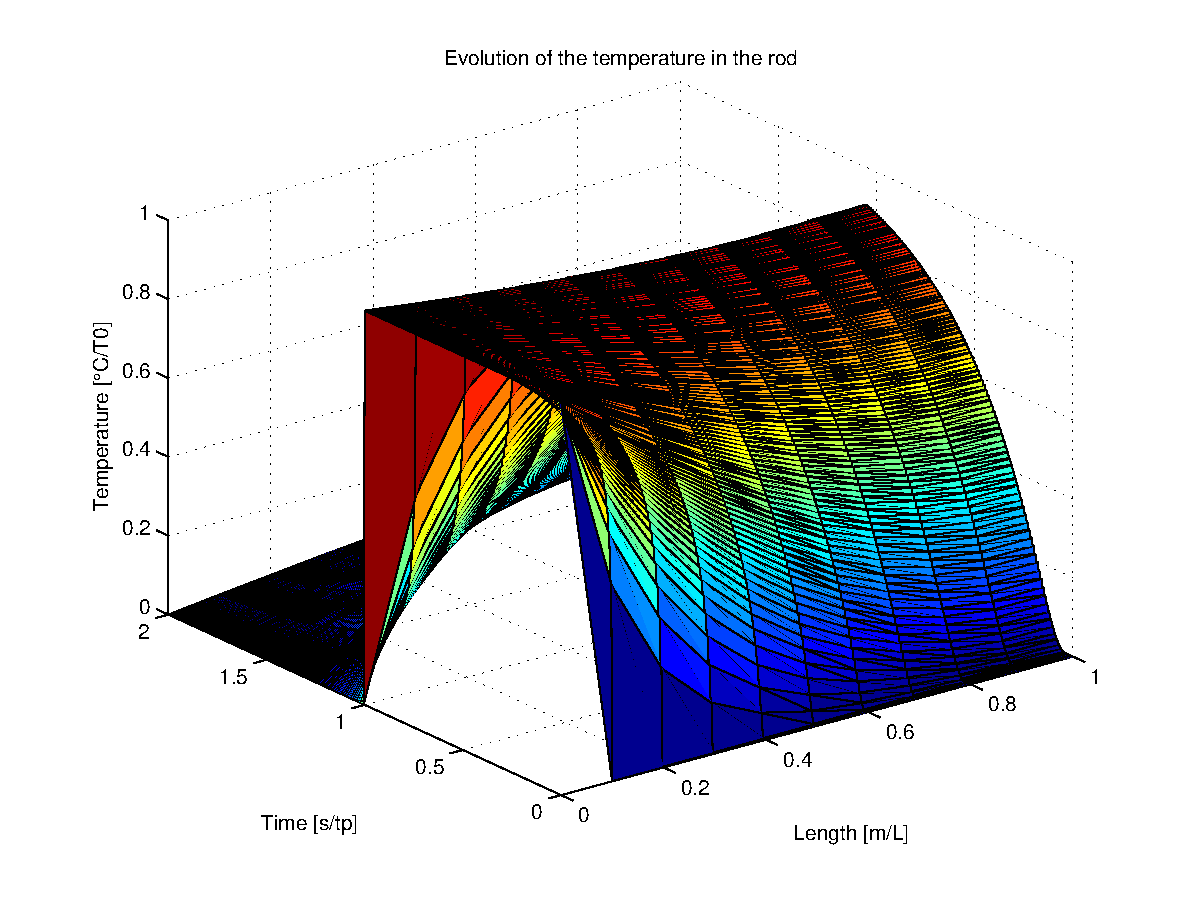
\includegraphics[width=0.7\textwidth]{stable.eps}
\caption{Temperature in the rod at any time}
\label{stable}
\end{center}
\end{figure}

\section*{Conclusion}
This report presented the solution of the very practical problem : the evolution of the temperature in a rod. This can be modelled as a parabolic PDE. To solve this PDE, we used the finite difference method to arrive at a system of ODEs. This system of ODE is stiff and a stiff method should then be used to solve it efficiently.

The stucture of the jacobian of the ODE system is really particular : it is tridiagonal (thus banded). This particularity should be taken into account when using the stiff solver (as did in section e) of the report).

\section*{MATLAB}
\lstinputlisting{graphics.m}
\lstinputlisting{tempEE.m}
\lstinputlisting{tempOde.m}


\end{document}